\chapter{The Value of Being Right}

Most pain is less solid than it feels.

A feeling can be intense and still be false. A mood can occupy the whole mind and still not describe the whole world. At certain moments a person may feel, with terrifying certainty, that the world has nothing to do with him. Yet that feeling is not a permanent truth. It is only a temporary state of attention.

The same is true of another common pain: the pain of being right and not being recognized.

Many people suffer because they believe they have seen something clearly, while others do not agree. They feel isolated, mocked, ignored, or delayed. The pain is real as a feeling, but the interpretation is often wrong. If you are right and almost no one agrees with you, you may not be standing in a tragedy. You may be standing near value.

The problem is that most people measure correctness by recognition. If many people agree, they feel safe. If few people agree, they feel anxious. This habit is understandable, but it is a poor instrument for judgment. The crowd can be right, but agreement itself is not proof. The crowd can be wrong, and disagreement itself is not failure.

Correctness by itself is not enough. Uniqueness by itself is not enough. The valuable condition is harder:

\begin{quote}
Be independent, be right, and be willing to act.
\end{quote}

\section*{Correctness Has a Second Dimension}

Most people think about being right along only one dimension: true or false, accurate or inaccurate, smart or foolish. That is too flat.

There is another dimension: how many other people already see the same thing.

If you are right, and everyone else is also right in the same way, your correctness has little commercial value. It may still be useful. It may protect you from error. It may help you avoid foolishness. But it does not give you much advantage, because there is no scarcity in the insight.

If you are wrong while everyone else is right, the situation is dangerous. You are not contrarian; you are simply mistaken.

If you are right while most others are wrong, the picture changes. Now the correctness has scarcity. It can become opportunity.

\begin{center}
\begin{adjustbox}{max width=\linewidth}
\begin{tabular}{p{0.22\linewidth}p{0.32\linewidth}p{0.32\linewidth}}
\hline
 & Others agree & Others disagree \\
\hline
You are wrong & Comfortable error & Isolated error \\
You are right & Common knowledge & Scarce insight \\
\hline
\end{tabular}
\end{adjustbox}
\end{center}

The lower right cell is where many important opportunities begin. It is also where discomfort begins, because human beings want safety from agreement.

The English word ``contrarian'' is often used for someone who moves against the crowd, especially in markets. But moving against the crowd is not valuable by itself. A person can oppose the crowd for vanity, anger, ignorance, or the pleasure of feeling special. That is not wisdom. It is merely reverse conformity.

The useful form is different:

\begin{quote}
Contrarian and correct.
\end{quote}

Even that is incomplete for our purposes. In this book, we need one more word:

\begin{quote}
Contrarian, correct, and active.
\end{quote}

Without action, the insight becomes a story you tell later at dinner: ``I knew it all along.'' That sentence is often the sound of wasted value.

\section*{The Simple Value Model}

A clean model helps:

\begin{center}
\begin{adjustbox}{max width=\linewidth}
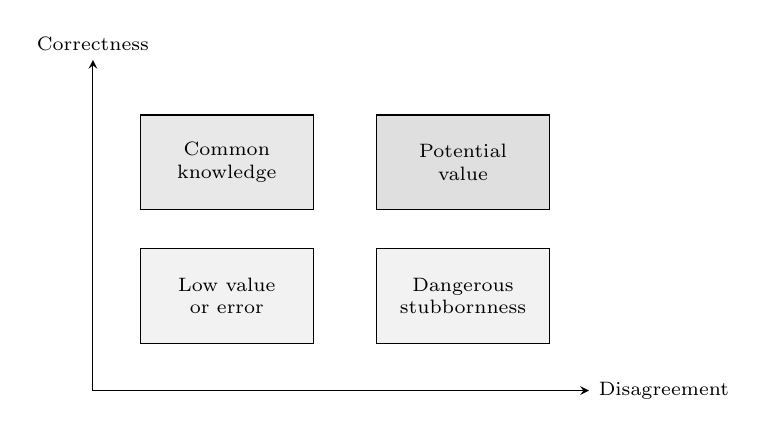
\begin{tikzpicture}[font=\scriptsize, >=stealth]
\draw[->] (0,0) -- (6.3,0) node[right] {Disagreement};
\draw[->] (0,0) -- (0,4.2) node[above] {Correctness};
\draw[fill=gray!10, draw] (0.6,0.6) rectangle (2.8,1.8);
\node[align=center] at (1.7,1.2) {Low value\\or error};
\draw[fill=gray!18, draw] (0.6,2.3) rectangle (2.8,3.5);
\node[align=center] at (1.7,2.9) {Common\\knowledge};
\draw[fill=gray!25, draw] (3.6,2.3) rectangle (5.8,3.5);
\node[align=center] at (4.7,2.9) {Potential\\value};
\draw[fill=gray!10, draw] (3.6,0.6) rectangle (5.8,1.8);
\node[align=center] at (4.7,1.2) {Dangerous\\stubbornness};
\end{tikzpicture}
\end{adjustbox}
\end{center}

This diagram is not mathematics. It is a guardrail for attention.

When your correctness is high and disagreement is high, the potential value is high. But the word ``potential'' is essential. You still need verification, execution, resources, timing, and endurance. Reality does not pay for private certainty. It pays for correct judgment converted into effective action.

A rough formula may be useful:

\begin{quote}
Value grows when correctness, scarcity of belief, and action multiply each other.
\end{quote}

If any one of the three is near zero, the result collapses.

Correctness without scarcity becomes ordinary competence.

Scarcity without correctness becomes delusion.

Correctness and scarcity without action become regret.

\section*{Why Disagreement Hurts}

If being right while others disagree may contain value, why do people suffer so much in that position?

Because most people are trained to be performance-oriented. They care less about whether something is truly good than about whether they look good. They care less about whether a judgment is correct than about whether agreement makes them feel safe.

To move with the majority is emotionally cheap. To think independently is expensive. It requires logic, patience, imagination, courage, and the ability to bear a period without applause. Most people do not merely lack these abilities. They have been rewarded for not using them.

In school, at work, and in families, agreement often receives quicker rewards than accuracy. A person learns to ask, ``What will make me look reasonable here?'' rather than, ``What is true?'' He learns to avoid embarrassment before he learns to test reality.

This produces a strange result. When a person finally finds a rare and correct view, he may treat the lack of agreement as evidence against the view. He becomes unhappy at the very signal that should make him more alert.

The better question is not:

\begin{quote}
Why does no one agree with me?
\end{quote}

The better question is:

\begin{quote}
Am I actually right, and if so, what action would let reality test it?
\end{quote}

That question returns attention from emotion to work.

\section*{Listening Without Obeying}

A wise rule from a former colleague expresses the balance well:

\begin{quote}
Listen to the majority, consult the minority, and finally decide for yourself.
\end{quote}

The first part does not mean obey the majority. It means listen. The majority reveals what most people believe, fear, ignore, repeat, and misunderstand. That information is useful. If many people are excited about an opportunity, competition may be fierce. If many people dismiss something, there may be hidden value or there may be a genuine trap. Either way, the crowd is data.

The second part matters too. Consult the minority. Find the few people who have studied the matter seriously. Find people with different incentives, different experiences, and different levels of skin in the game. Do not confuse loud disagreement with deep disagreement. A person who shouts against the crowd may still be shallow. A quiet practitioner may know more than both the crowd and the rebel.

Then decide for yourself. This is where responsibility enters. You cannot outsource the final judgment and still own the result. If you succeed, the consequence is yours. If you fail, the consequence is yours. This is why real independence requires courage. It is not a mood. It is willingness to bear the cost of one's own conclusion.

\section*{Four Examples}

The principle becomes clearer through concrete cases.

In 2003, almost everyone in China seemed to believe that preparing for TOEFL required at least twelve thousand words of vocabulary. It sounded authoritative because everyone repeated it. A careful statistical check suggested something different: after a certain base of school English vocabulary, roughly 2,142 additional words were enough for the core task. The difference between twelve thousand and 2,142 was not a small detail. It changed the learner's strategy, cost, confidence, and schedule.

That observation became the basis for a book on TOEFL core vocabulary that continued selling for years. The value did not come from being unusual for its own sake. It came from a correct conclusion that contradicted common belief and was turned into a product.

In 2007, another judgment appeared: most books on time management were wrong at the root. Time cannot be managed. Time passes at the same rate regardless of our preferences. What can be managed is the person, the team, the attention, the priorities, and the behavior inside time. That judgment became a book: \emph{Treat Time as a Friend}. Again, the value was not ``I disagree.'' The value was a more accurate frame, made usable for other people.

In 2011, Bitcoin looked strange, obscure, and difficult. At first it was not easy to understand. But the ability to read difficult material repeatedly, to finish what one does not yet understand, and to return until the structure becomes clearer, is a serious advantage. After enough study, the conclusion emerged: this thing is not nonsense. Then came discussions with smart people. Very few agreed. Among those few, even fewer were willing to act.

That combination was important: a conclusion that seemed increasingly correct, paired with very low agreement and even lower action. It suggested large potential value. The response was not to spend life persuading everyone. The response was to state the view publicly, then continue acting according to it.

In early 2015, another judgment formed: the era of free content on the internet was ending, and paid content was arriving. Friends listened politely. They did not strongly refute the idea, but they also did not act. That is a common form of disagreement: not argument, but inaction. By August 2015, a public account was opened. By November, paid communities and paid content products were being built. In July 2016, a paid column began and quickly gathered a large subscriber base. Later, major platforms moved into paid subscriptions.

The point is not that every such judgment will be right. The point is that value appeared only when judgment became action.

\section*{Action Separates Insight from Vanity}

There is a large difference between being independent in thought and being independent in conduct.

Independent thought is cheap enough to be common. People have unusual opinions all the time. They say, ``I think this will happen,'' or ``Everyone is wrong about that,'' or ``One day this will be big.'' Then nothing follows. No product, no investment, no study, no public commitment, no saved capital, no changed calendar, no trained skill.

Later, if the view proves right, they say, ``I knew it.'' But the market of reality did not buy the sentence. It rewards action under uncertainty, not commentary after certainty.

A useful test is severe:

\begin{quote}
If an idea is not correct enough for you to act on, you probably do not yet believe it enough.
\end{quote}

Action need not mean reckless all-in behavior. It may mean a small experiment, a written argument, a product prototype, a disciplined investment, a study plan, or a change in career direction. But some cost must be paid. Without cost, the idea remains entertainment.

This connects directly to attention. Attention is the first capital. To act on a rare correct view, you must reallocate attention away from easier pleasures: approval, debate, complaint, comparison, and proof of cleverness. The price of value is often paid first in attention.

\section*{The Trap of Self-Righteousness}

None of this is a license to become stubborn.

The difference between ``contrarian and correct'' and ``self-righteous'' is not tone. It is method.

Self-righteousness begins with identity: ``I am the kind of person who sees what others cannot see.'' From there, every disagreement becomes proof of superiority. Evidence is selected to protect the ego. Failed predictions are explained away. The person enjoys being different more than being accurate.

Independent correctness begins with reality: ``This conclusion appears true for these reasons, and I am willing to test it.'' From there, disagreement becomes data. Evidence is welcomed even when it hurts. Failed predictions are studied. The person cares more about becoming right than about appearing right.

The distinction can be made practical:

\begin{center}
\begin{tabular}{p{0.36\linewidth}p{0.46\linewidth}}
\hline
Self-righteousness & Independent correctness \\
\hline
Needs to look special. & Needs to understand reality. \\
Treats disagreement as insult. & Treats disagreement as information. \\
Collects supporters. & Collects evidence. \\
Avoids tests. & Seeks tests. \\
Uses being right as identity. & Uses being right as responsibility. \\
\hline
\end{tabular}
\end{center}

This is why metacognition remains central. The mind must watch not only the world, but also its own pleasure in being different. A person can become addicted to contrarianism. The addiction feels intellectual, but it is emotional.

\section*{Correct and Still Unrewarded}

Even when you are independent and correct, you are not guaranteed reward.

This is a difficult truth. Correctness is necessary in many situations, but it is not sufficient. Timing, capital, power, distribution, regulation, luck, and the actions of other people all matter.

Consider a painful case. Around 2013, many Bitcoin exchanges in China invited participation or investment on favorable terms. The refusal seemed logical: in a decentralized world, trying to build the largest center looked contradictory. The reasoning may have been correct. Yet in the following years, exchange businesses grew rapidly in valuation. Venture capital favored them. Their access to money, users, and market structure gave them advantages that an individual or a more logically elegant open-source approach could not easily match.

So a person can be right in one layer and still lose in another. He can understand a principle and underestimate capital scale. He can see a contradiction and miss the market's appetite. He can be correct too early, too small, too under-resourced, or too poorly positioned.

This does not destroy the principle. It completes it.

Being right is not magic. It is one variable in a wider system. The mature person accepts positive feedback without arrogance and negative feedback without collapse. If the world rewards him, he receives the reward calmly. If the world refuses or delays reward, he studies the refusal calmly.

That calm is courage.

\section*{Courage and Strategy}

The old phrase ``courage and strategy'' remains useful.

Courage means willingness to bear the consequences of one's own choice. Without courage, a person cannot truly be independent. He will retreat to consensus whenever the cost becomes visible. He may talk like a rebel, but he will act like a clerk of public opinion.

Strategy means respect for reality's structure. Without strategy, a person confuses emotion with insight. He charges against forces he has not studied. He mistakes stubbornness for principle. He ignores timing, incentives, resources, and the shape of the game.

Courage without strategy becomes reckless.

Strategy without courage becomes sterile.

Together, they make independent correctness more likely to become value.

\begin{center}
\begin{tabular}{p{0.28\linewidth}p{0.55\linewidth}}
\hline
Quality & Practical meaning \\
\hline
Courage & I accept the cost of my decision. \\
Strategy & I respect how reality actually works. \\
Action & I convert judgment into a test. \\
Calm & I accept feedback without distortion. \\
\hline
\end{tabular}
\end{center}

This is a demanding standard. That is precisely why it can produce value. If everyone could easily do it, the value would already be competed away.

\section*{Do Not Waste Correctness on Proving}

There is a hidden loss many smart people suffer for years: they use correctness to prove themselves instead of using it to grow.

The classroom offers a simple example. Some students are clever at finding faults in the teacher's words. Sometimes they are truly right. The teacher may have made a mistake, used a weak example, or skipped a condition. The student exposes it and feels victorious.

But what was the task? The task was not to prove that the student was right at that moment. The task was to learn, grow, and become more capable over time.

If attention is spent on proving, learning shrinks. The student wins a small social contest and loses a larger compounding opportunity. This kind of loss is especially dangerous because it may not be visible for years. The person remembers the moments of cleverness but not the growth he missed.

The better rule is:

\begin{quote}
Do not use correctness as a performance. Use correctness as a tool for growth.
\end{quote}

When you are right and others do not recognize it, ask what the situation is for. Is it for correction, action, research, patience, product creation, investment, or silence? Not every correct thought needs to be spoken. Not every spoken correction deserves a battle. Not every battle produces value.

Sometimes the highest use of being right is to shut up and build.

\section*{A Personal Audit}

The practice can be turned into a simple audit. When you believe you are right and others disagree, write down answers to these questions:

\begin{enumerate}
\item What exactly is my claim?
\item What evidence would prove me wrong?
\item Who disagrees, and what do they know that I may not know?
\item Is the disagreement real, or are people merely not acting?
\item If I am right, where is the practical value?
\item What small action can test the claim?
\item What cost am I willing to pay?
\item What feedback will I accept as reality's answer?
\end{enumerate}

This audit protects you from both cowardice and vanity. It prevents you from abandoning a valuable view too quickly merely because approval is absent. It also prevents you from worshiping your own opinion merely because it feels special.

The question is not, ``How can I make everyone admit I am right?''

The question is:

\begin{quote}
How can I turn a rare correct judgment into useful action while remaining open to correction?
\end{quote}

That is a wealth-freedom question. It joins attention, capital, time, execution, and metacognition into one practice.

\section*{The Pain Becomes a Signal}

Earlier, we saw that some pains are illusions. The feeling that the world has nothing to do with you is one such illusion. The world may not arrive preloaded with meaning, but meaning can be lived into it. Your actions create connections. Your attention leaves traces. Your work changes the degree to which the world becomes related to you.

The pain of being right without recognition can also be transformed.

If you treat disagreement as rejection, you suffer.

If you treat disagreement as possible evidence of scarce value, you investigate.

If investigation confirms that you are wrong, you have gained correction.

If investigation strengthens the view, you have gained a possible opportunity.

Either way, the pain has become useful.

This change can alter temperament. A person who understands the low value of mere correctness becomes less eager to argue. A person who understands the high value of rare correctness becomes less afraid of disagreement. A person who understands the necessity of action becomes less interested in showing off. A person who understands uncertainty becomes less arrogant.

He can think:

\begin{quote}
It is not important that I be recognized immediately. It is important that I become more accurate, act more effectively, and accept the result.
\end{quote}

This is freedom at the level of character.

To walk toward wealth freedom is not merely to collect money. It is to train the mind to notice value before it is popular, to build when applause is absent, to test ideas with reality, and to keep growing whether the first feedback is praise, silence, or a slap in the face.

Correctness alone may be worth little.

Correctness, scarcity, courage, strategy, action, and calm can be worth a life.
